\chapter{Probabilistic Generative Models}
In this part of the appendix, describes the Probabilistic Generative models (PGM) and how it is used on the dataset.

\section{Theory} 
The model is a multivariate normal distribution, which means that each class corresponds to a unique distribution.
\begin{equation}
p(\mathbf{x}|C_k)=\mathcal{N}(\mathbf{x};\mathbf{\mu}_k, \; \Sigma_k)
\end{equation}


\section{Results}

\subsection{1 digit:}

\begin{figure}[H]
\centering
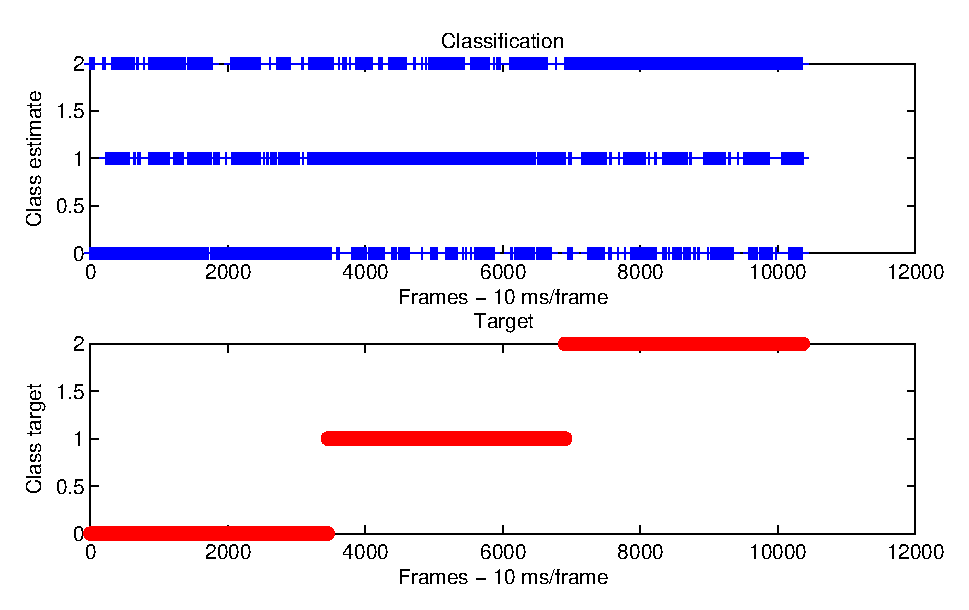
\includegraphics{PGM_1digit}
\caption{Results of using PGM classifiers and one digit spoken}
\label{fig:PGM_1dig}
\end{figure}

\begin{table}[H]                                                    
\centering                                                          
\begin{tabular}{|l|c|c|c|c|}                                        
\hline                                                              
  & Speaker Jacob & Speaker Mose & Speaker Simon & Precision [\%] \\
\hline                                                              
Estimate Jacob & 2027.0 & 313.0 & 391.0 & 74.2 \\                   
\hline                                                              
Estimate Mose & 569.0 & 2199.0 & 794.0 & 61.7 \\                    
\hline                                                              
Estimate Simon & 858.0 & 942.0 & 2269.0 & 55.8 \\                   
\hline                                                              
Sensitivity [\%] & 58.7 & 63.7 & 65.7 & 62.7 \\                     
\hline                                                              
\end{tabular}                                                       
\caption{Confusion matrix - 1 digit}                                
\label{table:PGM_conf_1}                                            
\end{table}       


\subsection{2 digits:}

\begin{figure}[H]
\centering
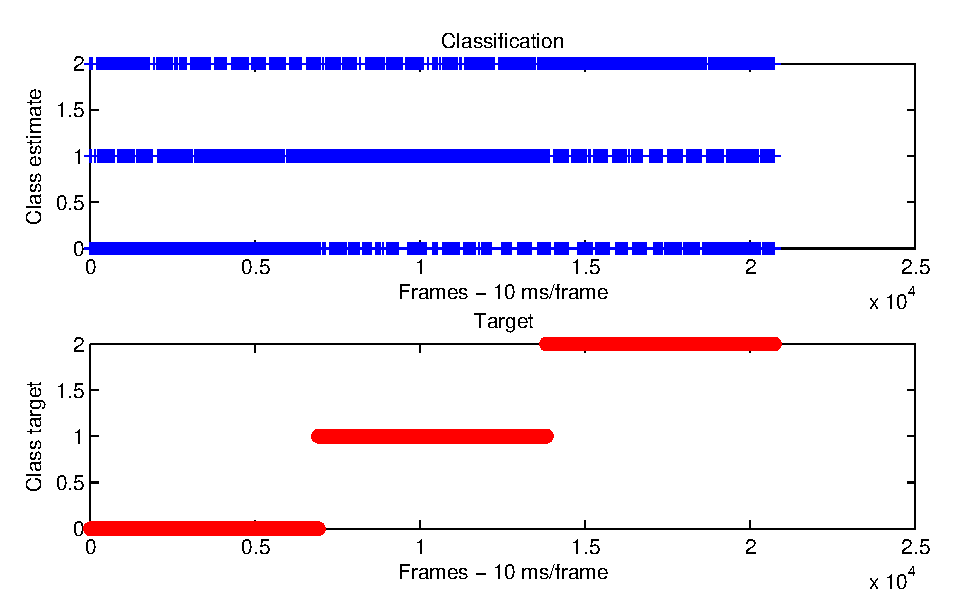
\includegraphics{PGM_2digit}
\caption{Results of using PGM classifiers and one digit spoken}
\label{fig:PGM_1dig}
\end{figure}

\begin{table}[H]                                                    
\centering                                                          
\begin{tabular}{|l|c|c|c|c|}                                        
\hline                                                              
  & Speaker Jacob & Speaker Mose & Speaker Simon & Precision [\%] \\
\hline                                                              
Estimate Jacob & 3471.0 & 585.0 & 1051.0 & 68.0 \\                  
\hline                                                              
Estimate Mose & 1567.0 & 4213.0 & 1500.0 & 57.9 \\                  
\hline                                                              
Estimate Simon & 1872.0 & 2112.0 & 4359.0 & 52.2 \\                 
\hline                                                              
Sensitivity [\%] & 50.2 & 61.0 & 63.1 & 58.1 \\                     
\hline                                                              
\end{tabular}                                                       
\caption{Confusion matrix - 2 digits}                               
\label{table:PGM_conf_2}                                            
\end{table}   


\subsection{10 digits:}

\begin{figure}[H]
\centering
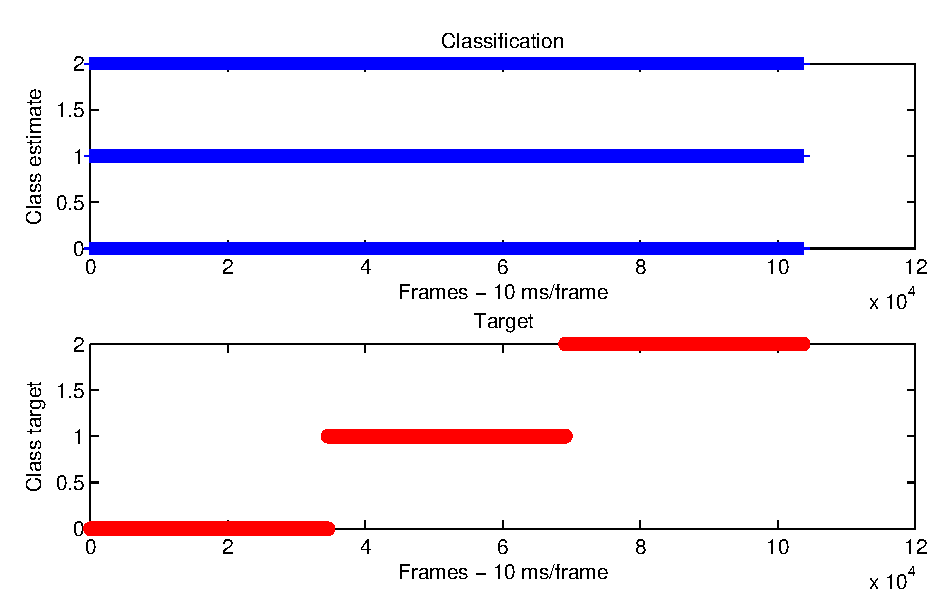
\includegraphics{PGM_10digit}
\caption{Results of using PGM classifiers and ten digits spoken}
\label{fig:PGM_10dig}
\end{figure}


\begin{table}[H]                                                    
\centering                                                          
\begin{tabular}{|l|c|c|c|c|}                                        
\hline                                                              
  & Speaker Jacob & Speaker Mose & Speaker Simon & Precision [\%] \\
\hline                                                              
Estimate Jacob & 18641.0 & 5089.0 & 5091.0 & 64.7 \\                
\hline                                                              
Estimate Mose & 9440.0 & 20760.0 & 9570.0 & 52.2 \\                 
\hline                                                              
Estimate Simon & 6478.0 & 8710.0 & 19898.0 & 56.7 \\                
\hline                                                              
Sensitivity [\%] & 53.9 & 60.1 & 57.6 & 57.2 \\                     
\hline                                                              
\end{tabular}                                                       
\caption{Confusion matrix - 10 digits}                              
\label{table:PGM_conf_10}                                           
\end{table} 